\documentclass[english,11pt]{article}
\usepackage[T1]{fontenc}
\usepackage[utf8]{inputenc}
\usepackage{graphicx}
\usepackage{geometry}
\usepackage{caption}
\usepackage{subcaption}
\usepackage{babel}
\usepackage{amsmath}
\usepackage[nottoc,numbib]{tocbibind}
\usepackage{verbatim}
\usepackage{pdfpages}
\usepackage{hyperref}
\usepackage{wrapfig}
\newcommand{\ok}{\fontsize{9}{11}\selectfont}

\newcommand{\listing}[1]{
    \subsection{#1}
    \label{lst:#1}
    {\small \verbatiminput{#1}}
}
\DeclareGraphicsExtensions{.png,.jpg,.pdf}

\begin{document}

\title{Advanced Networking and Communications 4\\
    Assessed Exercise 1}
\author{Motiejus Jakštys\\ 1003704}
\date{07 March 2013}

\maketitle
\tableofcontents

\clearpage

\section{Informal high-level overview of the application}

Application is written in ANSI C (C89) for maximum portability, using only
standard functions defined in POSIX specification.

The Application is divided into 3 modules:

\begin{description}
    \item[diagnostics.c] consists of functions for printing diagnostical
        data to the user. This includes routing tables and shortest routes.
    \item[msgqueue.c] has message queue implementation (application specific
        linked list).
    \item[main.c] is the main application, which has the UI and routing
        logic functions.
\end{description}

\subsection{How the application works}

First data is read from file which is given in command line: \texttt{argv[1]},
and the \texttt{ui} loop is called.

\section{How to use the program}
\subsection{How to build the executable}

A C89 compiler is needed. Most of the C compilers will work (MS Visual Studio,
GCC, Clang). If \texttt{Make} and a C compiler is present, this is enough to
build it:

\texttt{\$ make}

However, if \texttt{Make} is not present, one will have to explicitly compile
it. For example, with GCC:

\texttt{\$ gcc main.c msgqueue.c diagnostics.c -o main.exe}

\subsection{How to run the executable}

It needs a file with initial data as its first parameter, otherwise error
message will be displayed. Then a prompt will be provided for the user. For
example, to run it with \texttt{sample1.txt}:

{\ok
\begin{verbatim}
    $ main sample1.txt
    Enter your command (h for help):
    > h
    Commands
      s | z                - toggle split horizon
      m [from] [to] [cost] - modify link
      d [from] [to]        - delete link
      n                    - next iteration
      b [from] [to]        - print best route
      p                    - print routing table
      q | x                - quit
      h                    - this help
    Enter your command (h for help):
    >
\end{verbatim}
}

For example, to print the full routing table, enter \texttt{p}:

{\ok
\begin{verbatim}
Via  |  0  1  2  3  |  0  1  2  3  |  0  1  2  3  |  0  1  2  3  |
-----+--------------+--------------+--------------+--------------+
To 0 |  .  .  .  .  |  3  .  7  .  | 23  5  . 15  |  .  . 10  .  |
To 1 |  .  3 25  .  |  .  .  .  .  | 26  2  . 12  |  .  .  7  .  |
To 2 |  .  5 23  .  |  8  .  2  .  |  .  .  .  .  |  .  .  5  .  |
To 3 |  . 10 28  .  | 13  .  7  .  | 33  9  .  5  |  .  .  .  .  |
\end{verbatim}
}

How to interpret this output. These are routing tables of four nodes, delimited
by an \texttt{|}. Rows are destination nodes, and columns are the outgoing ports
(links) to reach the destination.

In this example, number "28" in table 1 means as follows: From node 0 (A) to
reach node 3 (D) one should go through node 2 (C), and the total cost via that
route is 28.

\section{Example network 1}

\begin{wrapfigure}{r}{0.3\textwidth}
    \label{img:sample1.png}
    \begin{center}
        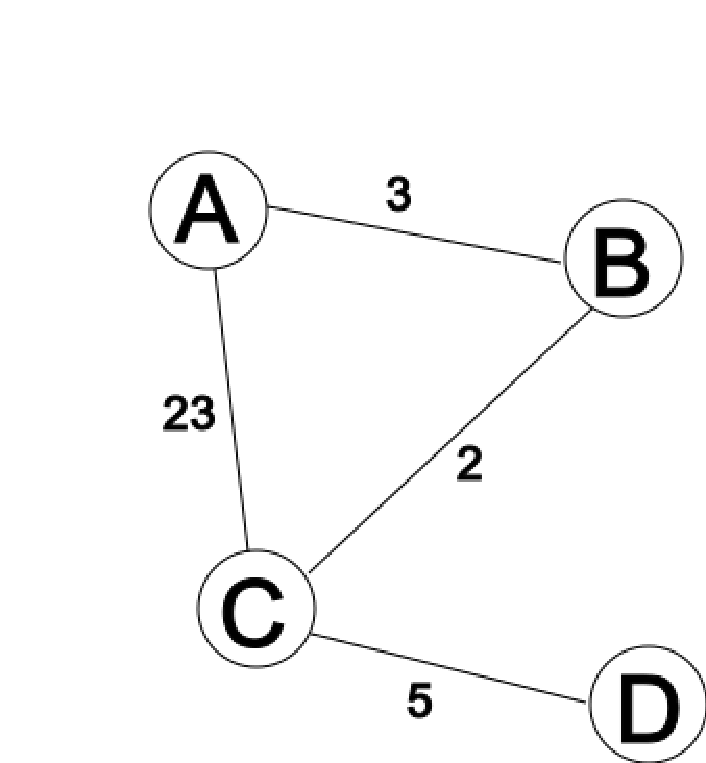
\includegraphics[width=0.25\textwidth]{sample1}
    \end{center}
    \caption{Sample1 network diagram}
\end{wrapfigure}

Routing table in \texttt{sample1.txt} is from a wikipedia entry about
Distance-vector routing protocol
\url{http://en.wikipedia.org/wiki/Distance-vector_routing_protocol}.

Mentioned wikipedia article had a minor error in the protocol demonstration,
which was fixed by me while programming the assessed exercise. See
reference~\cite{wpdiff} for a URL to see the fix.

\subsection{Example network 1 without split horizon}

Rundown is equivalent to wikipedia:

\clearpage
{\ok
\begin{verbatim}
$ ./main sample1.txt < cmdlist1_nohorizon.txt
Enter your command (h for help):
> p
Routing tables (0 to 3) after tick 0:
Via  |  0  1  2  3  |  0  1  2  3  |  0  1  2  3  |  0  1  2  3  |
-----+--------------+--------------+--------------+--------------+
To 0 |  .  .  .  .  |  3  .  .  .  | 23  .  .  .  |  .  .  .  .  |
To 1 |  .  3  .  .  |  .  .  .  .  |  .  2  .  .  |  .  .  .  .  |
To 2 |  .  . 23  .  |  .  .  2  .  |  .  .  .  .  |  .  .  5  .  |
To 3 |  .  .  .  .  |  .  .  .  .  |  .  .  .  5  |  .  .  .  .  |

Enter your command (h for help):
> n
Tick 1 iteration complete. Split horizon = 0. Not converged.
Enter your command (h for help):
> p
Routing tables (0 to 3) after tick 1:
Via  |  0  1  2  3  |  0  1  2  3  |  0  1  2  3  |  0  1  2  3  |
-----+--------------+--------------+--------------+--------------+
To 0 |  .  .  .  .  |  3  . 25  .  | 23  5  .  .  |  .  . 28  .  |
To 1 |  .  3 25  .  |  .  .  .  .  | 26  2  .  .  |  .  .  7  .  |
To 2 |  .  5 23  .  | 26  .  2  .  |  .  .  .  .  |  .  .  5  .  |
To 3 |  .  . 28  .  |  .  .  7  .  |  .  .  .  5  |  .  .  .  .  |

Enter your command (h for help):
> n
Tick 2 iteration complete. Split horizon = 0. Not converged.
Enter your command (h for help):
> p
Routing tables (0 to 3) after tick 2:
Via  |  0  1  2  3  |  0  1  2  3  |  0  1  2  3  |  0  1  2  3  |
-----+--------------+--------------+--------------+--------------+
To 0 |  .  .  .  .  |  3  .  7  .  | 23  5  . 33  |  .  . 10  .  |
To 1 |  .  3 25  .  |  .  .  .  .  | 26  2  . 12  |  .  .  7  .  |
To 2 |  .  5 23  .  |  8  .  2  .  |  .  .  .  .  |  .  .  5  .  |
To 3 |  . 10 28  .  | 31  .  7  .  | 51  9  .  5  |  .  .  .  .  |

Enter your command (h for help):
> n
Tick 3 iteration complete. Split horizon = 0. Route converged.
Enter your command (h for help):
> p
Routing tables (0 to 3) after tick 3:
Via  |  0  1  2  3  |  0  1  2  3  |  0  1  2  3  |  0  1  2  3  |
-----+--------------+--------------+--------------+--------------+
To 0 |  .  .  .  .  |  3  .  7  .  | 23  5  . 15  |  .  . 10  .  |
To 1 |  .  3 25  .  |  .  .  .  .  | 26  2  . 12  |  .  .  7  .  |
To 2 |  .  5 23  .  |  8  .  2  .  |  .  .  .  .  |  .  .  5  .  |
To 3 |  . 10 28  .  | 13  .  7  .  | 33  9  .  5  |  .  .  .  .  |
\end{verbatim}
}

I will not repeat wikipedia here, but in the end we end up with exactly the same
diagram.

However, there are a few problems. For instance, in the final route (final
table) node B to C via A has distance 8, which clearly does not make sense,
because it goes through A, while they are directly connected. To remedy the
problem, let's try the same network, but with split-horizon turned on:

{\ok
\begin{verbatim}

$ ./main sample1.txt < cmdlist1_horizon.txt
Enter your command (h for help):
> s
Split horizon = 1
Enter your command (h for help):
> n

    ...

Enter your command (h for help):
> n
Tick 3 iteration complete. Split horizon = 1. Route converged.
Enter your command (h for help):
> p
Routing tables (0 to 3) after tick 3:
Via  |  0  1  2  3  |  0  1  2  3  |  0  1  2  3  |  0  1  2  3  |
-----+--------------+--------------+--------------+--------------+
To 0 |  .  .  .  .  |  3  . 25  .  | 23  5  .  .  |  .  . 10  .  |
To 1 |  .  3 25  .  |  .  .  .  .  | 26  2  .  .  |  .  .  7  .  |
To 2 |  .  5 23  .  | 26  .  2  .  |  .  .  .  .  |  .  .  5  .  |
To 3 |  . 10 28  .  | 31  .  7  .  | 33  .  .  5  |  .  .  .  .  |
\end{verbatim}
}

As we can see, after introducing split-horizon this problem disappeared.

\section{Example network 2}

Let's try to converge this network:

\begin{figure}[h!]
    \label{img:sample1.png}
    \begin{center}
        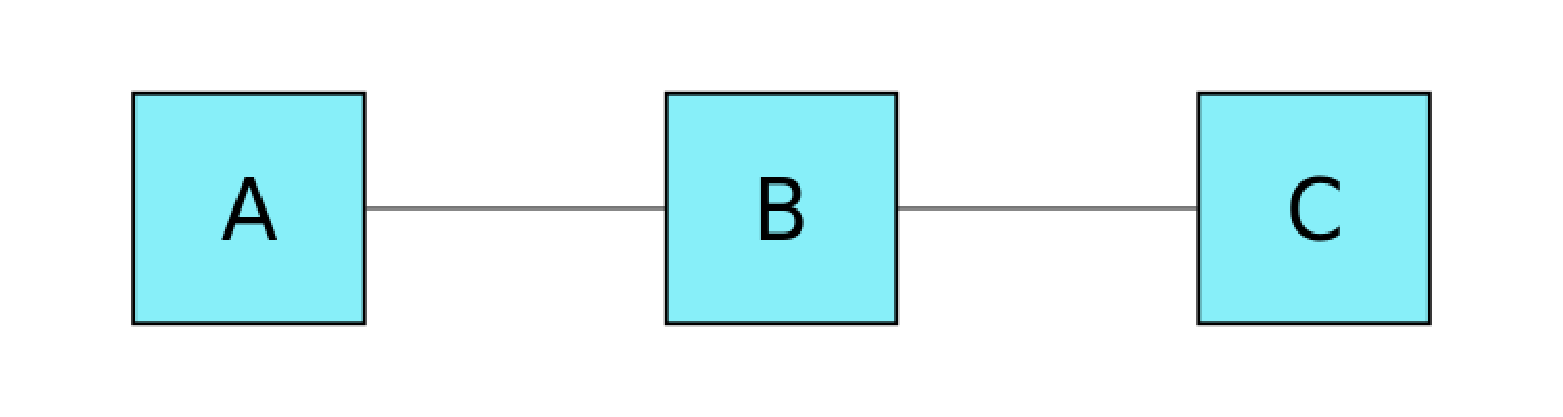
\includegraphics[width=0.5\textwidth]{sample2}
    \end{center}
    \caption{Sample2 network diagram}
\end{figure}

Distances between A and B and B and C are all 1.

We will make two tests: converge the network, remove link A-B, converge it again
and see what happens.

{\ok
\begin{verbatim}
Enter your command (h for help):
> n
Tick 1 iteration complete. Split horizon = 0. Not converged.
Enter your command (h for help):
> n
Tick 2 iteration complete. Split horizon = 0. Route converged.
Enter your command (h for help):
> p
Routing tables (0 to 2) after tick 2:
Via  |  0  1  2  |  0  1  2  |  0  1  2  |
-----+-----------+-----------+-----------+
To 0 |  .  .  .  |  1  .  3  |  .  2  .  |
To 1 |  .  1  .  |  .  .  .  |  .  1  .  |
To 2 |  .  2  .  |  3  .  1  |  .  .  .  |

Enter your command (h for help):
> d 0 1
Link dropped
Enter your command (h for help):
> n
Tick 3 iteration complete. Split horizon = 0. Route converged.
Enter your command (h for help):
> p
Routing tables (0 to 2) after tick 3:
Via  |  0  1  2  |  0  1  2  |  0  1  2  |
-----+-----------+-----------+-----------+
To 0 |  .  .  .  |  .  .  3  |  .  .  .  |
To 1 |  .  .  .  |  .  .  .  |  .  1  .  |
To 2 |  .  .  .  |  .  .  1  |  .  .  .  |
\end{verbatim}
}

As we can see, B still thinks it has a path to A via C (distance = 3), which is
wrong, because A is not connected to the network any more. Now same thing, but
with split horizon capability:
\clearpage

{\ok
\begin{verbatim}
Enter your command (h for help):                              
> z                                                           
Split horizon = 1                                             
Enter your command (h for help):                              
> n                                                           
Tick 1 iteration complete. Split horizon = 1. Not converged.  
Enter your command (h for help):                              
> n                                                           
Tick 2 iteration complete. Split horizon = 1. Route converged.
Enter your command (h for help):                              
> p                                                           
Routing tables (0 to 2) after tick 2:                         
Via  |  0  1  2  |  0  1  2  |  0  1  2  |                    
-----+-----------+-----------+-----------+                    
To 0 |  .  .  .  |  1  .  .  |  .  2  .  |                    
To 1 |  .  1  .  |  .  .  .  |  .  1  .  |                    
To 2 |  .  2  .  |  .  .  1  |  .  .  .  |                    
                                                              
Enter your command (h for help):                              
> d 0 1                                                       
Link dropped                                                  
Enter your command (h for help):                              
> n                                                           
Tick 3 iteration complete. Split horizon = 1. Route converged.
Enter your command (h for help):                              
> n                                                           
Tick 4 iteration complete. Split horizon = 1. Route converged.
Enter your command (h for help):                              
> p                                                           
Routing tables (0 to 2) after tick 4:                         
Via  |  0  1  2  |  0  1  2  |  0  1  2  |                    
-----+-----------+-----------+-----------+                    
To 0 |  .  .  .  |  .  .  .  |  .  .  .  |                    
To 1 |  .  .  .  |  .  .  .  |  .  1  .  |                    
To 2 |  .  .  .  |  .  .  1  |  .  .  .  |                    
\end{verbatim}
}


The problem is now solved and both B and C have correct routes to A.

\section{Conclusions and limitations}

I observed that the algorithm still converges incorrectly if there are cycles.
For example, removing link between D to C from sample1 will yield wrong routing
table for A, B and C even with split horizon capability. With sufficient time I
would improve the algorithm to take care of this case.

In some places efficiency was traded for clarity; this includes static-size
arrays (normally they should be unbounded and allocated on heap).

A real program would have no shared state, and components would be more modular
and decoupled. However, since the purpose of this application is
demonstrational, it is very convenient to modify global data structures without
passing too many pointers around.

\section{Source listings}
\listing{types.h}
\listing{diagnostics.h}
\listing{msgqueue.h}
\listing{diagnostics.c}
\listing{msgqueue.c}
\listing{main.c}

\clearpage
\begin{thebibliography}{9}

    \bibitem{wpdiff}
    \url{
    http://en.wikipedia.org/w/index.php?title=Distance-vector_routing_protocol&diff=542361426&oldid=540473569
    }

\end{thebibliography}
\end{document}
